\documentclass{amsart}
\usepackage{graphicx}
%\usepackage{tikzit}
\usepackage{dynkin-diagrams}
\usepackage[inkscapearea=page]{svg}
\svgpath{{inkscape/}}


\newif\ifshort
%\shorttrue
\shortfalse

\ifshort
%\usepackage[top=1.1in, bottom=1.1in, left=1.3in, right=1.3in]{geometry}
\usepackage[top=3.7cm, bottom=3.7cm, left=3.7cm, right=3.7cm]{geometry}
\pagestyle{plain}
\fi

% \usepackage{sty-en} 



\usepackage{tikz-cd, bm}
\usepackage{tikzit}

\usepackage{todonotes}
\newcommand\va[1]{\todo[color=green!40]{#1}} %valery
\newcommand\vainline[1]{\todo[inline,color=green!40]{#1}} %valery inline
\newcommand\ls[1]{\todo[color=orange!40]{#1}} %luca
\newcommand\lsinline[1]{\todo[inline,color=orange!40]{#1}} %luca inline
\newcommand\phil[1]{\todo[color=red!40]{#1}} %valery
\newcommand\philinline[1]{\todo[inline,color=red!40]{#1}} %valery inline

\usepackage[pdftex]{hyperref}
\hypersetup{colorlinks,citecolor=blue,linktocpage,hyperindex=true,backref=true}

\usepackage{etex}
\usepackage[utf8]{inputenc}
\usepackage{graphicx} 
\usepackage{amsfonts, amsmath, amssymb, amsthm, mathtools}
\usepackage[nameinlink]{cleveref}
\usepackage{mathrsfs, stmaryrd}
\usepackage{color}
\usepackage[english]{babel}
\usepackage{fontenc}
\usepackage{url}
\usepackage{bookmark}
\usepackage{caption}
\usepackage{subcaption}
\newdimen\figrasterwd
\figrasterwd\textwidth
\usepackage{epstopdf}
\usepackage{hyphenat}
\usepackage{float}
\usepackage{indentfirst}
\usepackage[export]{adjustbox}
\usepackage{pgfplots}
\usepackage{color}
\usepackage[all]{xy}\usepackage{array}
\newcolumntype{P}[1]{>{\centering\arraybackslash}p{#1}}
\usepackage{etoolbox}
\usepackage{quiver}
\usepackage{tikz}
\usetikzlibrary{arrows.meta, cd, fadings, patterns, calc, matrix, positioning, decorations, decorations.pathreplacing, decorations.markings, shapes, backgrounds, fit, shapes.geometric, intersections, hobby, matrix,arrows,decorations.pathmorphing}
\tikzfading[name=fade out, inner color=transparent!0, outer color=transparent!100]

\makeatletter
\def\maxwidth{\ifdim\Gin@nat@width>\linewidth\linewidth\else\Gin@nat@width\fi}
\def\maxheight{\ifdim\Gin@nat@height>\textheight\textheight\else\Gin@nat@height\fi}
\makeatother
% Scale images if necessary, so that they will not overflow the page
% margins by default, and it is still possible to overwrite the defaults
% using explicit options in \includegraphics[width, height, ...]{}
\setkeys{Gin}{width=\maxwidth,height=\maxheight,keepaspectratio}

% \bibliographystyle{amsalpha}
% \bibliography{references}
% \usepackage[
% style=alphabetic,
% sorting=ynt
% ]{biblatex}
% \addbibresource{references.bib}


\renewcommand{\hat}{\widehat}
% \renewcommand{\bar}{\overline}
\renewcommand{\tilde}{\widetilde}

\providecommand{\tightlist}{%
  \setlength{\itemsep}{0pt}\setlength{\parskip}{0pt}}

\usepackage{DZG_Style}
\usepackage{cleveref}
\usepackage{booktabs}
\usepackage{longtable}

%\usepackage{/home/dzack/Notes/tikzit}
\input{/home/dzack/Notes/sample.tikzstyles}



\title{Complete moduli spaces of Coble surfaces}
\date{August 18, 2024}
\author{D. Zack Garza}
\address{Department of Mathematics, University of Georgia, Athens GA 30602, USA}
\email{zack@uga.edu}

\usepackage[style=alphabetic,sorting=nyt]{biblatex} %Imports biblatex package
\addbibresource{/home/dzack/zotero.bib} %Import the bibliography file
\addbibresource{/home/dzack/CoblePaper.bib} %Import the bibliography file

\begin{document}

\begin{abstract}
We describe a modular KSBA stable pair compactification of the moduli space of Coble surfaces and compare it to a semitoroidal compactification of the corresponding period domain. We further describe KSBA stable limits in terms of integral affine structures.
\end{abstract}

\maketitle

\tableofcontents

\newpage

\section{Introduction}\label{introduction}

\begin{remark}

A Coble surface is a smooth projective rational surface \(S\) with \({\left\lvert {-K_S} \right\rvert} = \emptyset\) but \({\left\lvert {-2K_S} \right\rvert}\neq \emptyset\). Such surfaces arise from the work of \cite{Cob19} and \cite{Cob29} on Cremona transformations of \({\mathbf{P}}^2\) preserving an irreducible rational sextic \(C\) with ten nodes -- the blowup \(S\) along these nodes yields a Coble surface. \cite{Cob19} shows that the Cremona class of such a curve \(C\) can be written as a union of finitely many projective equivalence classes, and that if \(C\) is sufficiently general then \(\mathop{\mathrm{Aut}}(S) \cong W(E_{10})\), the Weyl group of an infinite root system of type \(E_{10}\). Moreover, he shows that that modulo \(\mathop{\mathrm{Aut}}(S)\), there are only finitely many smooth rational negative curves on \(S\).

Coble surfaces occur as degenerations of Enriques surfaces and were ultimately classified in \cite{DZ99}. As such, they are intimately tied to the theory of algebraic K3 surfaces equipped with a nonsymplectic involution, which were classified by \cite{nikulin1979quotient-groups}. For a reduced plane sextic \(C\), the double cover of \(S\) branched along the proper transform of \(C\) is a K3 surface \(X\) which can be realized as a degeneration of the universal double cover of an Enriques surface, where \(X\) acquires an \(A_1\) singularity fixed by the Enriques involution. The resulting quotient has a quartic singularity whose resolution is an irreducible smooth rational curve \(\tilde C\) satisfying \(\tilde C^2 = -4\), and thus by \cite[\S 3]{Nue16} is a Coble surface.

We will be interested in Coble surfaces in the strong sense, where \({\left\lvert {-2K_S} \right\rvert} = \left\{{C_1 + \cdots + C_n}\right\}\) is a single reduced divisor comprised of \(n\) disjoint smooth rational curves referred to as \emph{boundary components} of \(S\). It is known that \(1\leq n\leq 10\), and for each such \(n\), there is a moduli space \(F_{\Co, n}\) of Coble surfaces with \(n\) boundary components. When \(n=1\), the moduli space \(F_{\Co} \coloneqq F_{\Co, 1}\) of Coble surfaces can be described as a boundary divisor \(\cH_{-2}\) in the 10-dimensional moduli space \(F_{\operatorname{En}}\) of unpolarized Enriques surfaces, and thus \(F_{\Co}\) is 9-dimensional. Moreover, \(F_{\Co}\) was shown to be rational in \cite{DK13} via a comparison to a moduli space of cuspidal plane quintics. A natural question is whether or not \(F_{\Co}\) admits a geometrically meaningful, modular compactification \(\overline{F_{\Co}}\), and if so, if the boundary \(\partial \overline{F_{\Co}}\) can be described and classified. Toward this end, we turn to the stable pair compactifications of Kollár, Shepherd-Barron, and Alexeev \cite{kollar1988threefolds-and-deformations,alexeev1996moduli-spaces,Kol23}.

\end{remark}

\begin{remark}

The search for modular compactifications of moduli spaces is a central problem in algebraic geometry. The prototypical example stems from the work of \cite{deligne1969the-irreducibility-of-the-space, knudsen1976the-projectivity-of-the-moduli,knudsen1983the-projectivity-of-the-moduli23} on the Deligne-Mumford-Knudsen compactification \(\overline{{ \mathcal{M}_{g, n} }}\) of the moduli space of stable pointed curves \({ \mathcal{M}_{g, n} }\). By \cite{mumford1965git, namikawa1976a-new-compactification-of-the-siegel1, alexeev1999on-mumfords-construction, alexeev2002complete-moduli}, a similarly modular compactification \(\overline{{\mathcal{A}_g}}\) of the moduli space \({\mathcal{A}_g}\) of principally polarized abelian varieties via stable pairs exists, the normalization of which coincides with a particular choice of toroidal \cite{AMRT75} compactification by the work of \cite{kollar1988threefolds-and-deformations} and \cite{alexeev1996moduli-spaces}. By \cite{PSS71}, the coarse moduli space \(F_{2d}\) of primitively polarized K3 surfaces of degree \(2d\) is isomorphic to an arithmetic quotient \(D_{L_{2d}}/\Gamma_{L_{2d}}\) of a Type IV Hermitian symmetric domain associated to a lattice \(L_{2d}\), where \(D_{L_{2d}}\) is a period domain classifying Hodge structures of K3 type and \(\Gamma_{L_{2d}}\) is an arithmetic subgroup of the orthogonal group \({\operatorname{O}}(L_{2d})\). By \cite{BB66}, such domains admit a Baily-Borel compactification which is a projective variety. For \(F_{2d}\) and related lattice-polarized moduli spaces \(F_S\) of K3 surfaces, the boundary of the compactification consists of a configuration of 0-cusps (points) and 1-cusps (curves), see \cite{scattone1987on-the-compactification-of-moduli}. By \cite{AMRT75}, there additionally exist infinitely many toroidal compactifications described by a choice of fans at each cuspidal point of the Baily-Borel compactification. The work of \cite{looijenga1985semi-toric} on semitoroidal compactifications simultaneously generalizes the Baily-Borel and toroidal compactifications, retaining the advantage that the boundary can be understood in terms of semifans and studied using toric geometry.

Semitoroidal compactifications are advantageous due to their explicit and combinatorial nature, but do not a priori carry a clear modular interpretation along the boundary strata. Alternatively, letting \((S, R)\) be a pair consisting of a surface and a suitably chosen divisor, the work of \cite{kollar1988threefolds-and-deformations,alexeev1996moduli-spaces,Kol23} yields a compactification obtained by taking the closure of pairs \((S, \varepsilon R)\) in the space of KSBA stable pairs. Although KSBA compactifications admit strong modular interpretations, their boundary strata are generally quite difficult to describe. A recent strategy employed in \cite{alexeevCompactificationsModuliElliptic2023,AET23,AE22,AEGS23} is to simultaneously leverage the advantages of both semitoric and KSBA compactifications by finding comparison morphisms between them. This allows the modular boundary of the KSBA compactification to be studied and classified using the combinatorics of toric geometry, lattice theory, and critically, advances in integral affine geometry and mirror symmetry.

The moduli space \(F_\Co\) of Coble surfaces with \(n=1\) boundary components admits a Hodge-theoretic period domain description of the form \(D(T_\Co)/\Gamma_\Co\) where \(T_\Co\) is a fixed lattice and \(\Gamma_\Co \coloneqq{\operatorname{O}}(T_\Co)\) is its orthogonal group. Its Baily-Borel compactification \(\overline{F_{\Co}}^{\operatorname{BB}}\) contains only one 0-cusp \(p_0\), and thus the combinatorial data of a semitoroidal compactification is determined by a single \(\Gamma_\Co{\hbox{-}}\)invariant semifan associated to a lattice at \(p_0\). A canonical choice one can take is the Coxeter fan, formed by a fundamental domain of the action of the lattice's Weyl group, along with its reflections. Perhaps more naturally, one can also search for a semifan \({\mathcal{F}}\) such that the resulting compactification \(\overline{F_\Co}^{{\mathcal{F}}}\) is isomorphic to the KSBA compactification \(\overline{F_\Co}\) for a suitably chosen divisor, and indeed this is what we do in this paper. To this end, we prove the following:

\end{remark}

\begin{theorem}

There is a semifan \({\mathcal{F}}\) such that there exists a morphism \[
\Psi: (\overline{F_\Co})^{\nu} \to \overline{F_\Co}^{{\mathcal{F}}}
\] from the normalization of the KSBA compactification to the semitoroidal compactification associated with \({\mathcal{F}}\). The Coxeter fan of \(T_{\Co}\) is a refinement of \({\mathcal{F}}\), and stable Coble surfaces in the boundary of \(\overline{F_\Co}\) admit explicit descriptions in terms of surfaces associated to sub-Dynkin diagrams of Coxeter diagrams.

\end{theorem}

\begin{remark}

This result is made possible by recent advances in \cite{AE22,alexeev2021nonsymplectic} on compactifications of K3 surfaces with nonsymplectic automorphisms, along with the theory of recognizable divisors developed in \cite{alexeev2023compact}. We also critically leverage the related stable pair compactification of the moduli spaces of Enriques surfaces studied in \cite{AEGS23}. In particular, we use the folding theory of Coxeter diagrams, their associated integral affine structures, and the theory of \(ADE+BC\) surfaces in order to explicitly describe stable degenerations of Coble surfaces.

\end{remark}

\textbf{Acknowledgements}. I would like to thank my advisor Valery Alexeev for his guidance and support throughout this project. I thank Luca Schaffler and Philip Engel for many useful discussions. I would also like to gratefully acknowledge financial support from the Office of the Graduate School of the University of Georgia and the Research and Training Group in Algebra, Algebraic Geometry, and Number Theory at the University of Georgia.

\section{Coble surfaces}\label{coble-surfaces}

\subsection{The geometry of Coble surfaces}\label{the-geometry-of-coble-surfaces}

\begin{remark}

For the general theory of Coble surfaces, we refer to \cite{EnriquesOne,EnriquesTwo}, along with \cite{DM19, DZ99, dolgachev2013the-rationality, CD89, CD12, Dol17}. Following \cite[\S 5.1]{DM19}, a \textbf{Coble surface} is a smooth projective rational surface \(S\) with \({\left\lvert {-K_S} \right\rvert} = \emptyset\) but \({\left\lvert {-2K_S} \right\rvert} \neq \emptyset\). We say \(S\) is of \textbf{K3 type} if \({\left\lvert {-2K_S} \right\rvert}\) consists of a single smooth divisor \(C = C_1 + \cdots + C_n\), the union of \(n\) disjoint smooth rational curves satisfying \(C_i\cdot C_j = -4\delta_{ij}\). For Coble surfaces obtained as the blowup along ten nodes of a nodal plane sextic, this calculation follows from adjunction and the genus formula. We refer to \(C\) as the \emph{anti-bicanonical curve} of \(S\), and note that \(K_S\cdot C_i = -2\). The \(C_i\) are referred to as the \textbf{boundary components} of \(S\).

By \cite[\S 5.1]{Dol17}, such a Coble surface is known to be a \emph{basic rational surface}, i.e.~there is a birational morphism \(\pi: S\to {\mathbf{P}}^2\). Writing \(-K_S^2 = n\), one can decompose \(\pi\) as a blowup of \(N = 9+n\) points in \({\mathbf{P}}^2\). It is known that \(n\leq 10\), c.f. \cite[Prop.\,9.1.5]{EnriquesTwo}. The image of \(C\) is contained in \({\left\lvert {-2K_{{\mathbf{P}}^2}} \right\rvert} = {\left\lvert {{\mathcal{O}}_{{\mathbf{P}}^2}(6)} \right\rvert}\) and is thus generically a nodal plane sextic where the images of \(C_i\) are its irreducible components.

We will primarily be interested in the case \(n=1\), whence \(S\) is obtained as the blowup of a plane sextic along \(N=10\) ordinary double points, some of which may be infinitely near to each other. Such Coble surfaces are not the image of any birational but not biregular morphism from another Coble surface and are said to be \textbf{terminal}. We say \(S\) is \textbf{minimal} if the blowdown of any \((-1)\)-curve on \(S\) is no longer a Coble surface, or equivalently if \(S\) does not admit a birational but not biregular morphism onto another Coble surface.

\end{remark}

\begin{remark}

Let \(\cL \coloneqq{\mathcal{O}}_S(-K_S) \in \operatorname{Pic}(S)\); By \cite[Prop. 9.1.1]{EnriquesTwo}, taking a section \(s\in H^0(\cL ^{\otimes 2})\) with \(Z(s) = C\) yields a double branched double cover \(f: X\to S\) where \(X\) is a smooth K3 surface. By \cite[Def. 5.4.3]{EnriquesOne}, the preimages \(f^{-1}(C_i)\) are disjoint \((-2)\)-curves and \(\operatorname{Pic}(X)\) is a 2-elementary lattice with invariants of the form \[
(r,a,\delta)_1 = (10+n, 12-n, \delta)_1
.\] By \cite[Def. 5.4.3, Eqn. 5.3.1]{EnriquesOne}, the ramification divisor \(R\) is explicitly of one of the following forms:

\begin{itemize}
\tightlist
\item
  \(R=\emptyset\) if \((r,a,\delta) = (10, 10, 0)\),
\item
  \(R\) is a sum of two elliptic curves if \((r,a,\delta) = (10, 8, 0)\),
\item
  \(R\) is the sum of a single rational curve and \(n-1\) other disjoint \((-2)\)-curves otherwise.
\end{itemize}

It is also known that \(\delta=1\) unless \(n=8\), c.f. \cite[Table\, 5.1]{EnriquesOne}. Thus if \(S\) is a terminal Coble surface of K3 type with \(n=1\), the ramification locus of the K3 cover is a single smooth rational curve, and we obtain a lattice with invariants \[
S_{\Co} \coloneqq(11, 11, 1)_1 \cong \left\langle{-2}\right\rangle \oplus E_{10}(2)
\] with orthogonal complement \[
T_{\Co} \coloneqq S_{\Co}^{\perp \lkthree} = (11, 11, 1)_2 \cong \rm{I}_{2, 9}(2) \cong \left\langle{2}\right\rangle \oplus E_{10}(2)
.\]

Explicitly, \(S_{\Co}\) is generated by the preimages \(E_i\) for \(1\leq i \leq 10\) under \(f\) of the ten exceptional divisors of the blowup, along with the preimage \(E_0\) under \(f\) of the pullback of a hyperplane class of \({\mathbf{P}}^2\) under \(\pi\). One can show that \(E_0^2=2\) and \(E_i^2 = -2\) for \(i\geq 1\), and thus these divisors form a lattice of the form \[
S_{\Co} \cong \left\langle{2}\right\rangle \oplus \left\langle{-2}\right\rangle^{\oplus 10} \cong \rm{I}_{1, 10}(2) \cong (11, 11, 1)_1
,\] and the identification \(S_{\Co} \cong \left\langle{-2}\right\rangle \oplus E_{10}(2)\) follows from the fact that both definitions of \(S_{\Co}\) are 2-elementary lattices of signature \((1, 10)\) with discriminant group \((\bZ/2\bZ)^{11}\), which are classified uniquely up to isometry by their invariants \((r,a,\delta)_{n_+}\). Similarly, the identification of \(T_{\Co}\) follows from the fact that it is again a 2-elementary lattice of signature \((2, 9)\) satisfying \(q_{T_{\Co}} \cong -q_{S_{\Co}}\), and the isomorphism class of \(q_{T_{\Co}}\) determines \(T_{\Co}\) up to isometry. Alternatively, this can be seen directly using the mirror move \(S\leadsto T\) of \cite[Thm. 5.10]{AE22nonsympinv} applied to \(S_\Co =(11, 11, 1)_1\) in \cite[Fig.\,1]{AE22nonsympinv}, immediately yielding \(T_{\Co} = (11, 11, 1)_2\).

The lattices \(S_{\Co}\) and \(T_{\Co}\) will be of fundamental importance in constructing the Hodge-theoretic period domain for Coble surfaces, yielding a coarse space for the corresponding moduli space.

\end{remark}

\begin{remark}

Following \cite{CD12}, we note that this computation is a special case of a general construction. Let \(S\) be any basic rational surface and write \(S\) as the blowup of \({\mathbf{P}}^2\) at \(N\) points \(p_1,\cdots, p_N\) with \(N\geq 9\). It is a fact that \(\operatorname{Pic}(S) \cong \rm{I}_{1, N}\), since one can construct a \textbf{geometric basis} in the following way: let \(e_0\) be the class of the total transform of a hyperplane class in \({\mathbf{P}}^2\) and for \(1\leq i\leq N\), let \(e_i\) be the class of the total transform of the exceptional divisor over \(p_i\). Then \(\operatorname{Pic}(S) = \left\langle{e_0,e_1,\cdots, e_N}\right\rangle\) and \(\rho(X) = N+1\); one verifies that \(e_0^2 = 1\), and for \(i\geq 1\), that \(e_i^2 = -1\). Moreover \(e_ie_j = 0\) for \(i\neq j\), making this an orthogonal basis with respect to the intersection pairing, yielding \(\rm{I}_{1, N}\). In the case of Coble surfaces, the effect of taking the K3 double cover is to twist this lattice by 2, yielding \(\operatorname{Pic}(X) = \rm{I}_{1, N}(2)\), generated by preimages of the \(e_i\). We remark that \[
K_S = -3e_0 + e_1 + \cdots + e_N
.\]

\end{remark}

\section{Lattice Theory}\label{lattice-theory}

\begin{remark}

We refer to:

\begin{itemize}
\tightlist
\item
  \cite{vinberg1985hyperbolic-groups}
\item
  \cite{Vin75}
\end{itemize}

\end{remark}

\subsection{Basic Theory}\label{basic-theory}

\begin{remark}

The study of semitoroidal compactifications of moduli spaces of Coble surfaces largely reduces to lattice theory, of which we will now recall the essential notions.

\end{remark}

\begin{remark}[Basic invariants]

By a \textbf{lattice}, we mean a free \({\mathbf{Z}}\)-module \(L\) of finite rank equipped with a nondegenerate\footnote{A bilinear form is \emph{nondegenerate} if for any \(x\), \(\beta_L(x, L) = 0\) implies \(x=0\).} symmetric integral bilinear form \(\beta_L: L \otimes_{\mathbf{Z}}L \to {\mathbf{Z}}\). We abbreviate \(vw \coloneqq\beta_L(v, w)\) and \(v^2 \coloneqq\beta_L(v, v)\) and refer to the latter as the \textbf{norm} of \(v\). We write \(L_R \coloneqq L\otimes_{{\mathbf{Z}}} R\) and \(\beta_{L_R}\) for \(R = {\mathbf{Q}}, {\mathbf{R}}, {\mathbf{C}}\) for the \({\mathbf{Z}}\)-linear extensions of \((L, \beta_L)\) to the rational, real, and complex numbers respectively.

A submodule \(M\subseteq L\) is a \textbf{sublattice} if the restricted bilinear form \({ \left.{{\beta_L}} \right|_{{M}} }\) endows \(M\) with the structure of a lattice. A vector \(v\in L\) is \textbf{isotropic} if \(v^2 = 0\), i.e.~it is norm zero, and more generally a sublattice \(M \subseteq L\) is isotropic if \({ \left.{{\beta_L}} \right|_{{M}} } \equiv 0\). A lattice is said to be \textbf{even} if \(x^2\in 2{\mathbf{Z}}\) for all \(x\in L\), and \textbf{odd} otherwise. A nondegenerate symmetric bilinear form can be linearly extended to \(L_{\mathbf{R}}\) and by Sylvester's theorem, diagonalized with only \(1\) or \(-1\) on the diagonal. We write \(n_+\) and \(n_-\) respectively for the number of \(\pm 1\) entries on the diagonal. The \textbf{signature} of \(L\) is the pair \((n_+, n_-)\), and the \textbf{index} is \(n_+ - n_-\). We say \(L\) is \textbf{definite} if either \(n_+\) or \(n_-\) is zero, and \textbf{indefinite} otherwise. More precisely, if \(n_- = 0\) we say \(L\) is \textbf{positive definite}, and similarly if \(n_+ = 0\), we say \(L\) is \textbf{negative definite}. A negative definite lattice generated by elements of norm \(-2\) is said to be a \textbf{root lattice}, and such elements are referred to as \textbf{roots}.

The \textbf{rank} \(r\) of a lattice is its rank as a free \({\mathbf{Z}}\)-module and is given by \(r=n_+ + n_- = \dim_{\mathbf{Q}}L_{\mathbf{Q}}\). An indefinite lattice of signature \((1, r-1)\) is said to be \textbf{hyperbolic}. Fixing a generating set \(e_i\) of \(L\), we define the \textbf{Gram matrix} of \(L\) as the matrix \(G_L \coloneqq(\beta_L(e_i, e_j))_{ij}\), and the \textbf{discriminant} as \(\operatorname{disc} L \coloneqq\operatorname{det}G_L\). The discriminant is independent of the choice of generating set.

\end{remark}

\begin{remark}[Discriminant forms]

The \textbf{dual lattice} to \(L\) is denoted \(L {}^{ \vee }\coloneqq{ \operatorname{Hom} }_{\mathbf{Z}}(L, {\mathbf{Z}})\), and there is an morphism \[\begin{aligned}
\iota: L &\hookrightarrow L {}^{ \vee }\\
x &\mapsto \beta_L(x, \cdot)
\end{aligned}\] which, if \(L\) is nondegenerate, is an injection with finite index image. The \textbf{discriminant group} is \(A_L \coloneqq\operatorname{coker}\iota \cong L {}^{ \vee }/L\); this is a finite order group of order \({\left\lvert {\operatorname{disc} L} \right\rvert}\). We say \(L\) is \textbf{unimodular} if any of the following equivalent conditions hold:

\begin{enumerate}
\def\labelenumi{\arabic{enumi}.}
\item
  \(A_L\) is the trivial group,
\item
  \(\iota\) is an isomorphism and \(L\cong L {}^{ \vee }\),
\item
  \({\left\lvert { \operatorname{disc} L} \right\rvert} = 1\).
\end{enumerate}

If \(A_L \cong ({\mathbf{Z}}/p{\mathbf{Z}})^a\) for some \(a\), we say \(L\) is \textbf{\(p\)-elementary}; in our applications we will often have \(p=2\). For even lattices, the form \(\beta_L\) descends to a well-defined quadratic form \[\begin{aligned}
q_L: A_L &\to {\mathbf{Q}}/2{\mathbf{Z}}\\
x + L &\mapsto \beta_{L_{\mathbf{Q}}}(x, x) \operatorname{mod}2{\mathbf{Z}}
\end{aligned}\] We call the pair \((A_L, q_L)\) the \textbf{discriminant quadratic form} of \(L\). A \textbf{morphism} between two lattices is a morphism of \({\mathbf{Z}}\)-modules \(\eta: L\to L'\) respecting the bilinear forms in the sense that \(\beta_L(x, y) = \beta_{L'}(\eta(x), \eta(y))\), and is a \textbf{primitive embedding} if \(\eta\) is injective and \(\operatorname{coker}\eta\) is torsionfree. An \textbf{isometry} of lattices is an isomorphism, defined in the obvious way. We write \({\operatorname{O}}(L)\) for the group of lattice automorphisms of \(L\), denoted the \textbf{orthogonal group} of \(L\), and similarly \({\operatorname{O}}(q_L)\) for the \({\mathbf{Z}}\)-module automorphisms of of the discriminant form \(A_L\) which preserve the quadratic form. There is a natural group homomorphism \({\operatorname{O}}(L)\to{\operatorname{O}}(q_L)\), the kernel is denoted \(\tilde {\operatorname{O}}(L)\).

\end{remark}

\begin{remark}[Orthogonal complements]

Given two lattices \(L_1, L_2\) we write \(L_1\oplus L_2\) for the \textbf{orthogonal direct sum}, which is the direct sum of the underlying modules with bilinear form defined by \[\beta_{L_1\oplus L_2}(v_1 + v_2, w_1 + w_2)\coloneqq\beta_{L_1}(v_1, w_1) + \beta_{L_2}(v_2, w_2) 
.\] We write \(L^{\oplus n}\) for the direct sum of \(n\) copies of \(L\). Let \(\eta: M \hookrightarrow L\) be a primitive embedding of lattices, for example the inclusion of a sublattice. We write \[M^{\perp L} \coloneqq\left\{{x\in L \mathrel{\Big|}\beta_L(x, M) = 0}\right\}
.\] If the ambient lattice \(L\) is understood, we often abuse notation and simply write \(M^{\perp}\) without reference to \(L\). Note that \(M^{\perp L}\oplus M \subseteq L\) may not be saturated, and is generally a finite index sublattice of \(L\). We note that \(M^{\perp L}\cap M \neq \left\{{0}\right\}\) in general.\footnote{For example, let \(L = U = \left\langle{e,f}\right\rangle\) and \(M = \left\langle{e}\right\rangle\). Then \(M^{\perp L} = M\).} We also note that for any lattices \(L_i\), \[
A_{L_1 \oplus \cdots \oplus L_n} = A_{L_1} \oplus \cdots \oplus A_{L_n}
\]

\end{remark}

\begin{remark}[2-elementary lattices]

Let \(L\) be a 2-elementary lattice. The \textbf{divisibility} of a vector \(v\in L\), denoted \(\operatorname{div}_L(v)\), is defined by \(\beta_L(v, L) = \operatorname{div}_L(v){\mathbf{Z}}\), i.e.~the positive integral generator of the image of the map \(\beta_L(v, \cdot): L\to {\mathbf{Z}}\). For 2-elementary lattices, one always has \(\operatorname{div}_L(v) \in \left\{{1, 2}\right\}\). We set \(v^* \coloneqq v/\operatorname{div}_L(v)\in A_L\). Letting \(q_L:A_L \to {1\over 2}{\mathbf{Z}}/{\mathbf{Z}}\) be the induced quadratic form on \(A_L\), we say \(v^*\) is \textbf{characteristic} if \(q_L(x) = \beta_L(v^*, x)\operatorname{mod}{\mathbf{Z}}\) for all \(x\in A_L\), and is \textbf{ordinary} otherwise. We say that a primitive isotropic vector \(e\in L\) is

\begin{enumerate}
\def\labelenumi{\arabic{enumi}.}
\item
  \textbf{odd} if \(\operatorname{div}_L(e) = 1\),
\item
  \textbf{even ordinary} if \(\operatorname{div}_L(e) = 2\) and \(e^*\) is ordinary, or
\item
  \textbf{even characteristic} if \(\operatorname{div}_L(e) = 2\) and \(e^*\) is characteristic.
\end{enumerate}

The 2-elementary hyperbolic lattices admitting a primitive embedding into \(\Lambda_{\mathrm{K3}}\) were classified by Nikulin in \cite[\S 3.6.2]{nikulin1979integer-symmetric}. An indefinite 2-elementary lattice is determined up to isometry by a triple of invariants \((r,a,\delta)\). Here, \(r\coloneqq\operatorname{rank}_{\mathbf{Z}}(L)\) is the rank, \(a = \operatorname{rank}_{\bF_2}A_L\) is the exponent appearing in \(A_L = ({\mathbf{Z}}/2{\mathbf{Z}})^a\), and \(\delta \in \left\{{0, 1}\right\}\) is the \textbf{coparity}: we set \(\delta = 0\) if \(q_L(A_L) \subseteq {\mathbf{Z}}\), so \(q_L(x) \equiv 0 \operatorname{mod}{\mathbf{Z}}\) for all \(x\in A_L\), and \(\delta=1\) otherwise. We accordingly specify such lattices using the notation \((r,a,\delta)_{n_+}\).

\end{remark}

\begin{remark}[Twists of a lattice]

If \(L\) is a lattice with bilinear for \(\beta_L\), define \(L(n)\) to be the twist of \(L\) by \(n\), which has the same underlying \({\mathbf{Z}}\)-module but is equipped with the scaled bilinear form \[\beta_{L(n)}(v,w) \coloneqq n\cdot \beta_L(v, w).\]

\end{remark}

\begin{remark}[The lattice $\gens{n}$]

The lattice \(\left\langle{n}\right\rangle\) is defined as the rank 1 lattice \({\mathbf{Z}}\) with one generator \(v\) satisfying \(\beta_{\left\langle{n}\right\rangle}(v,v) = n\). The Gram matrix is the \(1\times 1\) matrix \(G_{\left\langle{n}\right\rangle} = [n]\), and the associated quadratic form is \(q_{\left\langle{n}\right\rangle}(x) = nx^2\).

\end{remark}

\begin{remark}[The hyperbolic lattice]

In rank 2, there are two unimodular hyperbolic lattices: the odd \(\rm{I}_{1, 1} \coloneqq\left\langle{1}\right\rangle \oplus \left\langle{-1}\right\rangle\), and the even \(U\coloneqq\rm{II}_{1, 1}\). We refer to the latter as the \textbf{hyperbolic lattice}, which can be realized as \(U \coloneqq{\mathbf{Z}}e \oplus {\mathbf{Z}}f\) with \(e^2=f^2 = 0\) and \(ef = 1\), and thus the following Gram matrix: \[ 
G_U = \begin{bmatrix}0&1\\1&0\end{bmatrix}
.\]

\end{remark}

\begin{remark}[ADE lattices]

Any Dynkin diagram of type \(A_n, D_n, E_6, E_7, E_8\) corresponds to a root lattice of the respective type. By convention, we take the negative definite twists of these lattices. Of particular importance to us is the \(E_8\) lattice associated to the following Dynkin diagram:

\begin{figure}[H]
\centering
\input{tikz/e8_coxeter_diagram.tikz}
\caption{The Dynkin diagram $E_{8}$}
\label{fig:e8-coxeter-diagram}
\end{figure}

\end{remark}

\begin{remark}[The lattice ${{\rm{I} }_{p, q}}$.]

For any pair of non-negative integers \((p, q)\), there exists an odd indefinite unimodular lattice determined up to isomorphism by its rank and signature: \[
\mathrm{I}_{p, q} \coloneqq\left\langle{1}\right\rangle^{\oplus p}\oplus \left\langle{-1}\right\rangle^{\oplus q}
.\]

\end{remark}

\begin{remark}[The lattice ${\rm{II}}_{p, q}$]

Let \(L\) be an even indefinite unimodular lattice of signature \((p, q)\). Then \(p-q\equiv 0 \pmod 8\), and \(L\) is uniquely determined up to isomorphism by its rank and signature: \[ 
{\rm{II}}_{p, q} \coloneqq
\begin{cases}
    U ^{\oplus p}\oplus E_8^{\oplus {q-p\over 8}}, & p < q \\
    U^{\oplus q} \oplus E_8(-1)^{\oplus {p-q\over 8}}, & p > q
.\end{cases}
\]

\end{remark}

\subsection{Summary}\label{summary}

\begin{remark}

We summarize the lattices that will be relevant to our discussion:

\[\begin{aligned}
    \lkthree &= (22, 0, 0)_3 = U^3 \oplus E_8^2 = \rm{II}_{3, 19} &
    E_{10} &= (10, 0, 0)_1 = U \oplus E_8 = \mathrm{I}_{1, 9} \\
    S_{\operatorname{En}} &= (10, 10, 0)_1    = E_{10}(2) & 
    T_{\operatorname{En}} &= (12, 10, 0)_2    = U \oplus E_{10}(2) \\
    S_{\Co} &= (11, 11, 1)_1    = \left\langle{-2}\right\rangle \oplus E_{10}(2) & 
    T_{\Co} &= (11,11,1)_2      = \left\langle{2}\right\rangle \oplus E_{10}(2) \\
    S_{\dP} &= (2,2,0)_1        = U(2) &
    T_{\dP} &= (20, 2, 0)_2     = U \oplus U(2) \oplus E_8^2
\end{aligned}\]

\end{remark}

\begin{lemma}

\label{lem:embedding_eta} Writing \begin{align*} T_{\Co} = \left\langle{2}\right\rangle \oplus E_{10}(2) &= \langle h, e', f',\alpha_1,\cdots, \alpha_8 \rangle \\ T_{\operatorname{En}} = U \oplus E_{10}(2) &= \langle \tilde e,\tilde f,\tilde e',\tilde f',\tilde \alpha_1,\cdots,\tilde \alpha_8\rangle, \end{align*} there is an embedding of lattices \(T_{\Co} \hookrightarrow T_{\operatorname{En}}\): \begin{align*}     \eta: \left\langle{2}\right\rangle \oplus E_{10}(2) &\to U \oplus E_{10}(2) \\     (h, x) &\mapsto (\tilde e + \tilde f, x) \end{align*} which sends the generator \(h\) of \(\left\langle{2}\right\rangle\) to \(\tilde e+\tilde f\in U\) and is the identity on the \(E_{10}(2)\) summand. Since \(\operatorname{coker}\eta\) is torsionfree, \(\eta\) is a primitive embedding.

\end{lemma}

\begin{lemma}

There is a sequence of primitive embeddings \[
T_{\Co} \hookrightarrow T_{\operatorname{En}} \hookrightarrow T_{\dP} \hookrightarrow\lkthree
\]\\
which is unique up to \({\operatorname{O}}(\lkthree)\). In particular, this yields an embedding \(T_{\Co}\hookrightarrow T_{\dP}\) given by \begin{align*}     \left\langle{2}\right\rangle \oplus U(2) \oplus E_8(2) &\hookrightarrow U \oplus U(2) \oplus E_8^2 \\     (h,x,y) & \mapsto (\tilde e + \tilde f, x, y, y) \end{align*} and thus an embedding \(F_{\Co} \hookrightarrow F_{(2,2,0)}\).

\end{lemma}

\begin{proof}

By \cite[Lem.\,2.4]{AEGS23}, it suffices to show uniqueness of \(S_{\operatorname{En}} \hookrightarrow S_{\Co}\), i.e. \[
E_{10}(2) \hookrightarrow\left\langle{-2}\right\rangle\oplus E_{10}(2)
,\] or equivalently by untwisting, \[
E_{10} \hookrightarrow\left\langle{-1}\right\rangle\oplus E_{10}
.\] This embedding is unique since one can write the codomain as \(E_{10}^\perp \oplus E_{10}\). Similarly, by \cite[Cor.\,1.5.2, Thm.\,3.6.3]{nikulin1979integer-symmetric}, the homomorphism \({\operatorname{O}}(L)\to {\operatorname{O}}(T_{\Co})\) is surjective.

\end{proof}

\begin{lemma}

\label{lem:lattice-embeddings-induce-morphisms} The embeddings of lattices \(\eta: T_{\Co}\hookrightarrow T_{\operatorname{En}}\) (resp. \(T_{\Co} \hookrightarrow T_{\dP}\)) induce locally closed embedding \(F_{\Co} \hookrightarrow F_{\operatorname{En}}\) (resp. \(F_{\Co} \hookrightarrow F_{(2,2,0)}\)) which extend to morphisms on the Baily-Borel compactifications.

\end{lemma}

\begin{proof}

This follows from \cite[\S 5, Thm.\,2]{kiernan1972satake-compactification}.

\end{proof}

\begin{theorem}

\(F_{\Co}\) is the normalization of a closed subvariety of \(F_{\operatorname{En}}\).

\end{theorem}

\begin{proof}

It suffices to show that \(D(T_{\Co})/{\operatorname{O}}(T_{\Co}) \to D(T_{\operatorname{En}})/{\operatorname{O}}(T_{\operatorname{En}})\) is a finite morphism which is generically injective. The lattice embedding \(T_{\Co}\hookrightarrow T_{\operatorname{En}}\) induces an injective morphism \(D(T_{\Co}) \hookrightarrow D(T_{\operatorname{En}})\). It remains to show that the stabilizer of \(T_{\Co}\) in \({\operatorname{O}}(T_{\operatorname{En}})\) is precisely \({\operatorname{O}}(T_{\Co})\) and the morphism is finite.

This morphism is finite because\ldots{}

The stabilizer statement follows from\ldots{}

\end{proof}

\todo[inline]{I don't know how to prove this. Maybe one should embed into $T_{\dP}$ instead to get the stabilizer statement? Finiteness is still unclear. Maybe one can use finite $\iff$ proper and finite fibers, using Stacks tag 02LS. This can be checked Zariski locally?}

\todo[inline]{Maybe this can be proved using Zariski's main theorem: a birational morphism to a normal variety with finite fibers is an isomorphism onto an open subset. Is this morphism birational? What are the fibers, and how can we tell if they are finite?}

\subsection{Moduli of Coble Surfaces}\label{moduli-of-coble-surfaces}

\begin{remark}

We begin with a naive parameter space for Coble surfaces. Following \cite{DK13}, by varying the coefficients of \(p_i\) in the planar blowup construction, one can construct \(F_\Co\) as a locally closed subvariety of \(({\mathbf{P}}^2)^{10}/\operatorname{PGL}_3\), which is of dimension \[
\dim ({\mathbf{P}}^2)^{10}/\operatorname{PGL}_3 = \dim ({\mathbf{P}}^2)^{10} - \dim \operatorname{PGL}_3 = 2\cdot 10 - (3^2-1) = 12
.\] A posteriori, the number of moduli for a Coble surface is 9, which means that there should be 3 conditions imposed upon the configuration of 10 points. These 3 conditions are precisely the \emph{discriminant conditions} described in \cite[\S 2,\,Prop. (10)]{Cob19}. Letting \(D\) be the corresponding discriminant locus, we can identify \(F_{\Co}\) as an open subset of \(\qty{ ({\mathbf{P}}^2)^{10} \setminus D }/\operatorname{PGL}_3\) at the level of coarse moduli spaces. We note that \cite{DK13} shows that \(F_\Co\) is rational by relating it to a codimension one subvariety of a moduli space of certain cuspidal quintics in \({\mathbf{P}}^2\).

\end{remark}

\begin{remark}

Alternatively, Horikawa \cite{Hor78b} and more recently \cite{AEGS23} consider the following: let \(Y\coloneqq{\mathbf{P}}^1\times {\mathbf{P}}^1\) and define an involution \(\tau(x,y) \coloneqq(-x,-y)\). Let \(B\in{\left\lvert {-2K_{Y}} \right\rvert}^\tau\) be a \(\tau\)-invariant anti-bicanonical curve in \(Y\). If \(B\) passes through a \(\tau\)-fixed point \(x,y\in \left\{{0, \pm \infty}\right\}\), then the corresponding double branched cover branched over \(B\) is a nodal K3 surface \(X\) with covering involution \(\iota_{\dP}\) such that \(Y = X/\left\langle{\iota_{\dP}}\right\rangle\). Letting \(\iota_{\operatorname{En}}\) be a lift of \(\tau\), the quotient \(Z\coloneqq X/\left\langle{\iota_{\operatorname{En}}}\right\rangle\) is a Coble surface. The case in which \(B\) does not pass through a \(\tau\)-invariant point yields an Enriques surface \(Z\), and an analysis of the corresponding moduli space is carried out in \cite{AEGS23}. In this way, one realizes the moduli space \(F_{\Co}\) of unpolarized Coble surfaces as a boundary divisor in \(F_{\operatorname{En}}\), the 10-dimensional moduli space of unpolarized Enriques surfaces.

\end{remark}

\begin{remark}

By passing to the K3 cover, one can embed \(F_\Co\) into an arithmetic quotient of a 9-dimensional Hermitian symmetric domain of type \(\rm{IV}\). Let \(\Lambda_{\mathrm{K3}}= U^3 \oplus E_8^2\) be the canonical K3 lattice. We recall that for any primitively embedded lattice \(S\hookrightarrow\Lambda_{\mathrm{K3}}\), letting \(T \coloneqq S^{\perp \Lambda_{\mathrm{K3}}}\), there is a Hodge-theoretic description of the coarse moduli space \(F_S\) of \(S\)-polarized K3 surfaces given by \[
F_S \coloneqq D_T/\tilde{\operatorname{O}}(T)
\] where \(\tilde {\operatorname{O}}(T) \coloneqq\ker\qty{{\operatorname{O}}(T) \to {\operatorname{O}}(q_T)}\) and \(D_T\) is a connected component of \[
\Omega_T \coloneqq\left\{{[v]\in {\mathbf{P}}(T_{\mathbf{C}}) {~\mathrel{\Big\vert}~}v^2=0,\, v\overline{v} > 0}\right\}
.\] Letting \(E_{10} \coloneqq U \oplus E_8\), one can consider the Enriques lattices \(S_{\operatorname{En}} := E_{10}(2)\) with \(T_{\operatorname{En}} \coloneqq U \oplus E_{10}(2)\). Letting \[
\cH_{-2d} = \bigcup_{\delta^2 = -2d} \delta^{\perp D_T}
.\] We note, as in \cite{DK13}, that \(T_{\Co} \cong v^{\perp T_{\operatorname{En}}}\) for some \(v^2=-2\), which implies that there is a birational isomorphism \(F_{\Co} \overset{\sim}{\dashrightarrow}\cH_{-2}/{\operatorname{O}}(T_{\operatorname{En}})\). Thus up to birational isomorphism, one can present \begin{align*} F_{\operatorname{En}} &= \qty{D_{T_{\operatorname{En}}} \setminus \cH_{-2}} / \tilde {\operatorname{O}}(T_{\operatorname{En}}) \\ F_{\Co} &= \cH_{-2} / \tilde {\operatorname{O}}(T_{\operatorname{En}}) \\ \end{align*} where surfaces along the divisor \(\cH_{-2}\) in \(F_{\operatorname{En}}\) correspond precisely to Coble surfaces. We note that surfaces along \(\cH_{-4}\setminus \cH_{-2}\) correspond to nodal Enriques surfaces, an interesting divisor in its own right.

\end{remark}

\begin{remark}

We summarize the relevant moduli spaces: \begin{align*} F_{\operatorname{En}} &= D_{T_{\operatorname{En}}}/\tilde {\operatorname{O}}(T_{\operatorname{En}}) &  F_{\operatorname{En}, 2} &= D_{T_{\operatorname{En}}}/\Gamma_{\operatorname{En}, 2} \\ F_\Co &= D_{T_{\Co}} / \tilde {\operatorname{O}}(T_{\Co}) &  F_{\Co, 2} &= D_{T_{\Co}}/\Gamma_{\Co, 2}  \end{align*} where \begin{align*} \Gamma_{\operatorname{En}, 2} &= {\operatorname{O}}(T_{\operatorname{En}}) \cap{\operatorname{O}}(T_\dP) \subseteq {\operatorname{O}}(\Lambda_{\mathrm{K3}}) \\ \Gamma_{\Co, 2} &= \mathrm{Stab}_{{\operatorname{O}}(T_{\operatorname{En}})}(T_{\Co}) \subseteq {\operatorname{O}}(T_{\operatorname{En}}) \end{align*} where \(T_{\dP}\) is described in \cite{AEGS23}. Note that we implicitly use the embedding \(\eta: T_{\Co} \hookrightarrow T_{\operatorname{En}}\) of \cref{lem:embedding_eta}.

\end{remark}

\begin{remark}

By \cref{lem:lattice-embeddings-induce-morphisms}, there are morphisms \(\overline{F_{\Co}}^{\operatorname{BB}} \to \overline{F_{\operatorname{En}}}^{\operatorname{BB}}\) and \(\overline{F_{\Co}}^{\operatorname{BB}} \to \overline{F_{(2,2,0)}}^{\operatorname{BB}}\) which induce correspondences between the boundary cusps.

\end{remark}

\begin{remark}

We set up the moduli space of KSBA stable pairs for Coble surfaces, possibly using the ramification divisor of the K3 involution (which is in this case not fixed-point free). The above embeddings should allow us to take closures of stable pairs in already existing moduli spaces.

\end{remark}

\section{Cusp Correspondence}\label{cusp-correspondence}

\subsection{Coble Cusps}\label{coble-cusps}

\begin{remark}

We recall the mirror move algorithm from \cite{AE22nonsympinv}. We have Nikulin's 2-elementary diagram:

\begin{figure}[H]
\centering
\input{tikz/nikulin_table.tikz}
\caption{White nodes are $\delta=0$, black are $\delta=1$, double circled are $\delta = 1,2$.}
\label{fig:nikulin_table}
\end{figure}

\end{remark}

\begin{remark}

Having identified the 2-elementary lattice \(S_\Co = (11, 11, 0)_1\), one can apply the mirror move algorithm of \cite[Thm. 5.10]{AE22nonsympinv} to determine the 0-cusps and 1-cusps of \(F_\Co\). The outcome of the algorithm is summarized by the following tree:

\begin{figure}[H]
\centering
\begin{tikzcd}[row sep=large, column sep=0.65em]
% https://q.uiver.app/#q=WzAsMTUsWzUsNSwiKDcsIDcsIDEpXzAiLFsyMjIsMTAwLDYwLDFdXSxbNSwxLCIoMTEsIDExLCAxKV8yIl0sWzUsMywiKDksIDksIDEpXzEiLFsyMjIsMTAwLDYwLDFdXSxbNiw1LCIoNywgNywgMClfMCIsWzAsNjAsNjAsMV1dLFs4LDUsIlxcYnVsbGV0Il0sWzksNSwiXFxidWxsZXQiXSxbMTAsNSwiXFxidWxsZXQiXSxbMiw1LCJcXGJ1bGxldCJdLFsxLDUsIlxcYnVsbGV0Il0sWzksMywiKDksIDksIDApXzEiLFswLDYwLDYwLDFdXSxbMCw1LCJcXGJ1bGxldCJdLFsxLDMsIig5LCAxMSwgMSlfMSIsWzAsNjAsNjAsMV1dLFs0LDUsIig3LDksMSlfMCIsWzAsNjAsNjAsMV1dLFs1LDAsIigxMSwgMTEsMSlfMSJdLFs1LDQsIlxcYnVsbGV0Il0sWzEsMl0sWzEsOV0sWzEsMTFdLFsxMSwxMF0sWzExLDhdLFsxMSw3XSxbMiwxMl0sWzIsMF0sWzIsM10sWzksNV0sWzksNF0sWzksNl0sWzEzLDFdXQ==
	&&&&& {(11, 11,1)_1} \\
	&&&&& {(11, 11, 1)_2} \\
	\\
	& \textcolor{rgb,255:red,214;green,92;blue,92}{(9, 11, 1)_1} &&&& \textcolor{rgb,255:red,51;green,112;blue,255}{(9, 9, 1)_1} &&&& \textcolor{rgb,255:red,214;green,92;blue,92}{(9, 9, 0)_1} \\
	&&&&&  \\
	\bullet & \bullet & \bullet && \textcolor{rgb,255:red,214;green,92;blue,92}{(7,9,1)_0} & \textcolor{rgb,255:red,51;green,112;blue,255}{(7, 7, 1)_0} & \textcolor{rgb,255:red,214;green,92;blue,92}{(7, 7, 0)_0} && \bullet & \bullet & \bullet
	\arrow[from=1-6, to=2-6]
	\arrow[from=2-6, to=4-2]
	\arrow[from=2-6, to=4-6]
	\arrow[from=2-6, to=4-10]
	\arrow[from=4-2, to=6-1]
	\arrow[from=4-2, to=6-2]
	\arrow[from=4-2, to=6-3]
	\arrow[from=4-6, to=6-5]
	\arrow[from=4-6, to=6-6]
	\arrow[from=4-6, to=6-7]
	\arrow[from=4-10, to=6-9]
	\arrow[from=4-10, to=6-10]
	\arrow[from=4-10, to=6-11]
\end{tikzcd}

\caption{Blue (resp. red) indicate lattices which are valid (resp. invalid) targets of mirror moves.}
\label{fig:unlabeledtwo}
\end{figure}

Thus \(F_{\Co}\) has one 0-cusp corresponding to an isotropic vector \(v\) with \[
v_0^{\perp T_{\Co}}/\left\langle{v_0}\right\rangle \cong (9,9,1)_1 \cong \left\langle{2}\right\rangle \oplus E_{8}(2)
.\] Moreover, this 0-cusp \(v_0\) is incident to one 1-cusp \(C_0\) corresponding to an isotropic plane \(J = \left\langle{v_0, v_1}\right\rangle\) with \[
J^{\perp T_{\Co}}/\left\langle{J}\right\rangle \cong (7,7,1)_0 \cong A_1^{\oplus 7}
.\] where \(v_1 \in v_0^{\perp T_{\Co}}/\left\langle{v_0}\right\rangle\). In the diagrammatic language of \cite[Fig.\, 1, Thm.\,5.10]{AE22nonsympinv}, this corresponds to a \(U^2\) move and can be summarized in the following mirror move diagram as a composition of two even ordinary \(U(2)\)-type moves:

\begin{figure}[H]
\centering
\begin{tikzpicture}[decoration=snake]

\node[style=black node 
	,label={[label distance=0.75em]-90: $(11,11,1)_1$}
	,label={[label distance=0.75em]90: $S$}
] (p1) at (0, 0) {};
\node[style=black node 
	,label={[label distance=0.75em]-90: $(11,11,1)_2$}
	,label={[label distance=0.75em]90: $T$}
] (p2) at (2, 0) {};
\node[style=black node 
	,label={[label distance=0.75em]-90: $(9,9,1)_1$}
	,label={[label distance=0.75em]90: $\bar T$}
] (p3) at (4, 0) {};
\node[style=black node 
	,label={[label distance=0.75em]-90: $(7,7,1)_0$}
	,label={[label distance=0.75em]90: $\bar{\bar{T}}$}
] (p4) at (6, 0) {};

%\draw[shorten >= 0.2em, decorate] (p1) to (p2.west);
\draw[-latex, shorten >= 0.4em, style=double] (p2) to (p3.west);
\draw[-latex, shorten >= 0.4em, style=double] (p3) to (p4.west);

\draw [-latex,decorate, ->]
(0.2,0) -- (1.8,0);

\node at (2.75, 0.20) {$U(2)$};
\node at (4.75, 0.20) {$U(2)$};

\end{tikzpicture}
\caption{}
\label{fig:unlabeledthree}
\end{figure}

Note that \(v_0\) corresponds to a Type \(\rm{III}\) boundary, while \(C_0\) corresponds to a type \(\rm{II}\) boundary. It is easily verified that the Coxeter diagram \(G_{(9,9,1)_1}\) at \(v_0\) has precisely one maximal parabolic subdiagram, corresponding to a finite-index root lattice of type \(A_7\). We note that by \cite[\S 5]{AE22nonsympinv}, such isotropic vectors are unique up to \({\operatorname{O}}(T_\Co)\), and so we can choose representatives:

\begin{itemize}
\tightlist
\item
  \(v_0 = e'\),
\item
  \(v_1 = 2h + \alpha_1 + \alpha_2\).
\end{itemize}

Calculations verify that \(v_0^2 = v_1^2 = 0\), that \(v_1 \in v_0^{T_{\Co}}/\left\langle{v_0}\right\rangle\), and that \(v_0v_1 = 0\), and thus \(J \coloneqq\left\langle{v_0, v_1}\right\rangle\) is an admissible choice of an isotropic plane. We further note that \(\operatorname{div}_{T_{\Co}}(v_0) = \operatorname{div}_{T_{\Co}}(v_1) = 2\), which will be an important invariant for establishing a correspondence to cusps of other moduli spaces. For an isotropic plane \(J\), we denote the divisibilities of the constituent generating vectors as a tuple \((d_1, d_2)\), and in this convention we have \(\operatorname{div}_{T_{\Co}}(v_0, v_1) = (2, 2)\). We summarize this in the following boundary cusp diagram:

\begin{figure}[H]
\centering
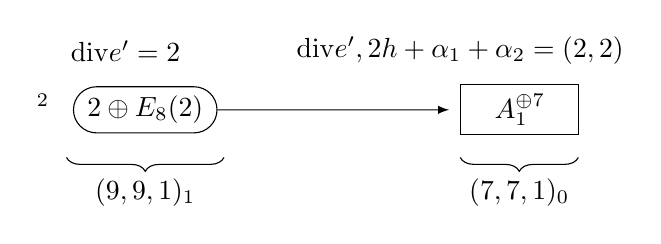
\begin{tikzpicture}
    \node [rounded rectangle, draw,
    label={[label distance=0.5em]180: $\bD^2$}
    ] (v0) at (0, 0) {$\gens{2} \oplus E_{8}(2)$};
    \node [rectangle, draw, minimum width=1.5cm, anchor=west] (C0) at (4,0) {$A_1^{\oplus 7}$};
    \draw[-latex, shorten >= 0.4em] (v0) to (C0.west);

\draw [decorate,decoration={brace,amplitude=5pt,mirror,raise=4ex}]
  (-1,0) -- (1,0) node[midway,yshift=-3em]{$(9,9,1)_1$};

\draw [decorate,decoration={brace,amplitude=5pt,mirror,raise=4ex}]
  (4,0) -- (5.5,0) node[midway,yshift=-3em]{$(7,7,1)_0$};

\node at (-0.25,0.75) {$\mathrm{div}\gens{e'} = 2$};

\node at (4,0.75) {$\mathrm{div}\gens{e',  2h+\alpha_1+\alpha_2} = (2, 2)$};

    \end{tikzpicture}

\caption{Cusp diagram for $F_\Co = F_{(11, 11, 1)}$ where $T_\Co = \left\langle{2}\right\rangle \oplus E_{10}(2)$.}
\label{fig:coble-cusp-diagram}
\end{figure}

\end{remark}

\begin{remark}

As further proof that this cusp diagram is correct, we can use the theory of Coxeter diagrams. Given an isotropic vector \(e\in L\) a lattice of signature \((2, n)\), the lattice \(e^{\perp L}/\left\langle{e}\right\rangle\) is a hyperbolic lattice equipped with a root system \(R_e\) with a Coxeter diagram \(G_e\). Generally, when \(e\) corresponds to a 0-cusp in a Baily-Borel compactification, the adjacent 1-cusps correspond precisely to maximal parabolic subdiagrams of \(G_e\). The cusp diagram above suggests that the 0-cusp \(v_0\) should have a Coxeter diagram \(G_{v_0}\) with precisely one maximal parabolic subdiagram. One can run Vinberg's algorithm to determine the Coxeter diagram for \(v_0\), and it is a straightforward check to determine that there is indeed a unique maximal parabolic subdiagram of the form \(\tilde B_7(2)\):

\begin{figure}[H]
\centering
\begin{tikzpicture}[row sep=large, column sep=small]
  
    \node [style=black node] (1) at (0, 0) {};
    \node at (0, -0.3) {$1$};
    
    \node [style=black node] (3) at (1, 0) {};
    \node at (1, -0.3) {$3$};
    
    \node [style=black node] (4) at (2, 0) {};
    \node at (2, -0.3) {$4$};
    
    \node [style=black node] (2) at (2, 1) {};
    \node at (2, 1.3) {$2$};
    
    \node [style=black node] (5) at (3, 0) {};
    \node at (3, -0.3) {$5$};
    
    \node [style=black node] (6) at (4, 0) {};
    \node at (4, -0.3) {$6$};
    
    \node [style=black node] (7) at (5, 0) {};
    \node at (5, -0.3) {$7$};
    
    \node [style=black node] (8) at (6, 0) {};
    \node at (6, -0.3) {$8$};
    
    \node [style=white node] (9) at (7, 0) {};
    \node at (7, -0.3) {$9$};
    
    \node at (5, 1) {$\tilde B_7(2) \subset G_{(9, 9, 1)_1}$};
    
    
    \draw (1) to (4);
    \draw (4) to (2);
    \draw (4) to (8);
    \draw [style=double edge] (8) to (9);
    
    \begin{pgfonlayer}{background}
    \fill[cyan,opacity=0.2] \convexpath{3,9}{8pt};
    \fill[cyan,opacity=0.2] \convexpath{2,4}{8pt};
    \fill[cyan,opacity=0.2] \convexpath{3,4}{8pt};
    \end{pgfonlayer}
    
    \end{tikzpicture}

\caption{The unique maximal parabolic subdiagram $\tilde B_7(2)$ of $(9,9,1)_1$, corresponding to single one-cusp $(7,7,1)_0$ in $F_\Co$.}
\label{fig:coble-cusp-9-9-1-parabolics}
\end{figure}

\end{remark}

\begin{remark}

\begin{align*} \operatorname{div}_{T_{\dP}}(v_0) = 2 && \operatorname{div}_{T_{\dP}}(v_1) = 1  .\end{align*}

The former is clear, since the image of \(v_0\) in \(T_{\dP}\) is \(e'\in U(2)\) and \(e'f' = 2\). The latter follows from the fact that \(v_1\alpha_3 = 1\).

\end{remark}

\begin{remark}

We note the divisibilities of \(v_i\) under various lattice embeddings:

\begin{table}[H]
\centering
\begin{tabular}{|l|l|l|l|l|}
\hline
Coble Vector & Representative & $\mathrm{div}_{T_{\Co}}$ & $\mathrm{div}_{T_{\operatorname{En}}}$ & $\mathrm{div}_{T_{\dP}}$ \\ \hline
$v_0$        & $e'$   & 2                        & 2                        & 2                        \\ \hline
$v_1$        & $2h + \alpha_1 + \alpha_2$   & 2                        & 2                        & 1                        \\ \hline
\end{tabular}
\caption{Isotropic vectors in $F_{\operatorname{En}, 2}$ and their divisibilities.}
\label{tab:sterk-cusps-two}
\end{table}

More concisely:

\begin{table}[H]
\centering
\begin{tabular}{|l|l|l|l|}
\hline
Lattice   & Image of $v_0$ & Image of $v_1$                  & Divisibility \\ \hline
$T_{\Co}$ & $e'$           & $2h + \alpha_1 + \alpha_2$      & $(2, 2)$     \\ \hline
$T_{\operatorname{En}}$ & $e'$           & $2e + 2f + \alpha_1 + \alpha_2$ & $(2, 2)$     \\ \hline
$T_{\dP}$ & $e'$ & $2e + 2f + \alpha_1 + \tilde\alpha_1 + \alpha_2 + \tilde \alpha_2$ & $(2, 1)$ \\ \hline
\end{tabular}
\caption{Isotropic vectors in $F_{\operatorname{En}, 2}$ and their divisibilities.}
\label{tab:coble-cusp-divisibilities}
\end{table}

\end{remark}

\subsection{Enriques Cusps}\label{enriques-cusps}

\begin{remark}

We recall the cusp diagram of \(F_{\operatorname{En}}\):

\begin{figure}[H]
\centering
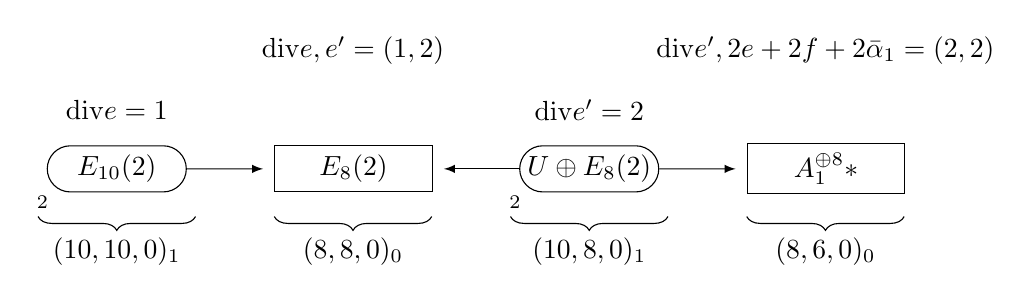
\begin{tikzpicture}
\node [rounded rectangle, draw, minimum width=2cm
	, label={[label distance=0.01em]200: $\RP^2$}
] (w0) at (0, 0) {$E_{10}(2)$};

\node [rectangle, draw, anchor=west,
minimum width=2cm
] (C12) at (2,0) {$E_8(2)$};

\node [rounded rectangle, draw, minimum width=2cm
	, label={[label distance=0.01em]200: $\bD^2$}
] (w1) at (6, 0) {$U \oplus E_8(2)$};

\node [rectangle, draw, anchor=west,
minimum width=2cm
] (C2) at (8,0) {$A_1^{\oplus 8}*$};
    %%%%
    \draw[-latex, shorten >= 0.4em] (w0) to (C12.west);
    \draw[-latex, shorten >= 0.4em] (w1) to (C12.east);
    \draw[-latex, shorten >= 0.4em] (w1) to (C2.west);


\node at (0,0.75) {$\mathrm{div}\gens{e} = 1$};
\draw [decorate,decoration={brace,amplitude=5pt,mirror,raise=4ex}]
  (-1,0) -- (1,0) node[midway,yshift=-3em]{$(10,10,0)_1$};

\node at (3,1.5) {$\mathrm{div}\gens{e, e'} = (1, 2)$};
\draw [decorate,decoration={brace,amplitude=5pt,mirror,raise=4ex}]
  (2,0) -- (4,0) node[midway,yshift=-3em]{$(8,8,0)_0$};

\node at (6,0.75) {$\mathrm{div}\gens{e'} = 2$};
\draw [decorate,decoration={brace,amplitude=5pt,mirror,raise=4ex}]
  (5,0) -- (7,0) node[midway,yshift=-3em]{$(10,8,0)_1$};

\node at (9,1.5) {$\mathrm{div}\gens{e', 2e+2f+2\bar\alpha_1} = (2, 2)$};
\draw [decorate,decoration={brace,amplitude=5pt,mirror,raise=4ex}]
  (8,0) -- (10,0) node[midway,yshift=-3em]{$(8,6,0)_0$};

    \end{tikzpicture}

\caption{Cusp diagram for $F_{\operatorname{En}} = F_{(10, 10, 0)}$ corresponding to $T_{\operatorname{En}} = U \oplus E_{10}(2)$.}
\label{fig:enriques-cusp-diagram}
\end{figure}

This can be recovered using the mirror move algorithm:

\begin{figure}[H]
\centering
\begin{tikzpicture}[decoration=snake]

\node[style=white node] (p1) at (0, 0) {};

\node[style=white node] (p2) at (2, 0) {};

\node[style=white node] (p3) at (4, 2) {};

\node[style=white node] (p4) at (4, -2) {};

\node[style=white node] (p5) at (6, 0) {};

\node[style=white node] (p6) at (6, -2) {};



%\draw[shorten >= 0.2em, decorate] (p1) to (p2.west);
\draw[-latex, shorten >= 0.4em] (p2) to (p3.west);
\draw[-latex, shorten >= 0.4em, style=double] (p2) to (p4.west);

\draw[-latex, shorten >= 0.4em, style=double] (p3) to (p5.west);
\draw[-latex, shorten >= 0.4em] (p4) to (p5.west);

\draw[-latex, shorten >= 0.4em, style=double] (p4) to (p6.west);


\draw [-latex,decorate, ->]
(0.2,0) -- (1.8,0);

\node at (3.25, .75) {$U$};
\node at (4.7, 0.75) {$U(2)$};

\node at (3.25, -.75) {$U(2)$};
\node at (4.7, -0.75) {$U$};

\node at (4.7, -2.25) {$U(2)$};


\node at (0, 3) {$S$};
\node at (2, 3) {$T$};
\node at (4, 3) {$\bar{T}$};
\node at (6, 3) {$\bar{\bar{T}}$};

\node at (-0.5, 0.5) {$(10, 10, 0)_1$};
\node at (1.5, 0.5) {$(12, 10, 0)_2$};

\node at (3.5, 2.5) {$(10, 10, 0)_1$};
\node at (3.5, -2.5) {$(10, 8, 0)_1$};

\node at (6.5, 0.5) {$(8, 8, 0)_0$};
\node at (6.5, -1.5) {$(8, 6, 0)_0$};

\end{tikzpicture}
\caption{}
\label{fig:mirror-moves-enriques-simplified}
\end{figure}

\end{remark}

\begin{remark}

We recall the Coxeter diagrams and their maximal parabolic subdiagrams at the 0-cusps of \(F_{\operatorname{En}}\):

\begin{figure}[H]
\centering
\caption{}
\begin{tikzpicture}[scale=0.8]
\begin{scope}[shift={(0,-1.25)}]
\node [style=black node] (1) at (0, 0) {};
\node at (0, -0.3) {$1$};

\node [style=black node] (3) at (1, 0) {};
\node at (1, -0.3) {$3$};

\node [style=black node] (4) at (2, 0) {};
\node at (2, -0.3) {$4$};

\node [style=black node] (2) at (2, 1) {};
\node at (2, 1.3) {$2$};

\node [style=black node] (5) at (3, 0) {};
\node at (3, -0.3) {$5$};

\node [style=black node] (6) at (4, 0) {};
\node at (4, -0.3) {$6$};

\node [style=black node] (7) at (5, 0) {};
\node at (5, -0.3) {$7$};

\node [style=black node] (8) at (6, 0) {};
\node at (6, -0.3) {$8$};

\node [style=black node] (9) at (7, 0) {};
\node at (7, -0.3) {$9$};

\node [style=black node] (10) at (8, 0) {};
\node at (8, -0.3) {$10$};

\draw (1) to (4);
\draw (4) to (2);
\draw (4) to (10);

\node at (6, 1) {$\tilde E_8(2) \subset (10, 10, 0)_1$};

\begin{pgfonlayer}{background}
\fill[cyan,opacity=0.2] \convexpath{1,9}{8pt};
\fill[cyan,opacity=0.2] \convexpath{2,4}{8pt};
\end{pgfonlayer}
\end{scope}

\begin{scope}[shift={(9,0)}]

\node [style=black node] (1) at (0, 0) {};
\node at (0, -0.3) {$1$};

\node [style=black node] (3) at (1, 0) {};
\node at (1, -0.3) {$3$};

\node [style=black node] (4) at (2, 0) {};
\node at (2, -0.3) {$4$};

\node [style=black node] (2) at (2, 1) {};
\node at (2, 1.3) {$2$};

\node [style=black node] (5) at (3, 0) {};
\node at (3, -0.3) {$5$};

\node [style=black node] (6) at (4, 0) {};
\node at (4, -0.3) {$6$};

\node [style=black node] (7) at (5, 0) {};
\node at (5, -0.3) {$7$};

\node [style=black node] (8) at (6, 0) {};
\node at (6, -0.3) {$8$};

\node [style=black node] (9) at (7, 0) {};
\node at (7, -0.3) {$9$};

\node [style=white node] (10) at (8, 0) {};
\node at (8, -0.3) {$10$};

\draw (1) to (4);
\draw (4) to (2);
\draw (4) to (9);
\draw [style=double edge] (9) to (10);

\node at (6, 1) {$\tilde E_8(2) \subset (10, 8, 0)_1$};

\begin{pgfonlayer}{background}
\fill[cyan,opacity=0.2] \convexpath{1,3,4}{8pt};
\fill[cyan,opacity=0.2] \convexpath{2,4}{8pt};
\fill[cyan,opacity=0.2] \convexpath{4,9}{8pt};
\end{pgfonlayer}

\end{scope}

\begin{scope}[shift={(9,-2.5)}]

\node [style=black node] (1) at (0, 0) {};
\node at (0, -0.3) {$1$};

\node [style=black node] (3) at (1, 0) {};
\node at (1, -0.3) {$3$};

\node [style=black node] (4) at (2, 0) {};
\node at (2, -0.3) {$4$};

\node [style=black node] (2) at (2, 1) {};
\node at (2, 1.3) {$2$};

\node [style=black node] (5) at (3, 0) {};
\node at (3, -0.3) {$5$};

\node [style=black node] (6) at (4, 0) {};
\node at (4, -0.3) {$6$};

\node [style=black node] (7) at (5, 0) {};
\node at (5, -0.3) {$7$};

\node [style=black node] (8) at (6, 0) {};
\node at (6, -0.3) {$8$};

\node [style=black node] (9) at (7, 0) {};
\node at (7, -0.3) {$9$};

\node [style=white node] (10) at (8, 0) {};
\node at (8, -0.3) {$10$};

\draw (1) to (4);
\draw (4) to (2);
\draw (4) to (9);
\draw [style=double edge] (9) to (10);

\node at (6, 1) {$\tilde B_8(2) \subset (10, 8, 0)_1$};

\begin{pgfonlayer}{background}
\fill[cyan,opacity=0.2] \convexpath{3, 10}{8pt};
\fill[cyan,opacity=0.2] \convexpath{2,4}{8pt};
\end{pgfonlayer}

\end{scope}

\end{tikzpicture}

\label{fig:enriques-maximal-parabolics-10-10-0}
\end{figure}

\end{remark}

\subsection{Sterk Cusps}\label{sterk-cusps}

\begin{remark}

We recall Sterk's cusp diagram for \(F_{\operatorname{En}, 2}\):

\begin{figure}[H]
\centering

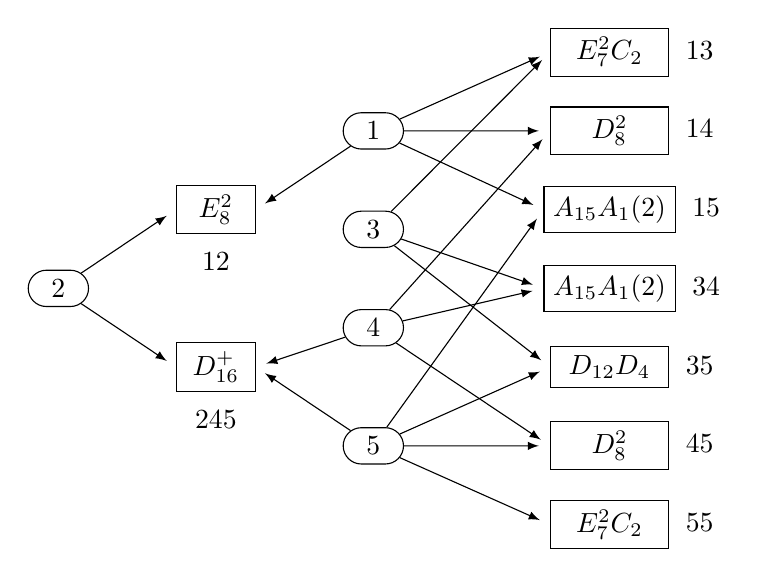
\begin{tikzpicture}

\node[rounded rectangle, draw,minimum width=1cm] (v2) at (0, 0) {$2$};

\node[rectangle, draw,minimum width=1cm,label={[label distance=0.25em]-90: $12$}] (C12) at (2, 1) {$E_8^2$};
\node[rectangle, draw,minimum width=1cm,label={[label distance=0.25em]-90: $245$}] (C245) at (2, -1) {$D_{16}^+$};


\node[rounded rectangle, draw,minimum width=1cm] (v1) at (4, 2) {$1$};
\node[rounded rectangle, draw,minimum width=1cm] (v3) at (4, .75) {$3$};
\node[rounded rectangle, draw,minimum width=1cm] (v4) at (4, -0.5) {$4$};
\node[rounded rectangle, draw,minimum width=1cm] (v5) at (4, -2) {$5$};

\node[rectangle, draw,minimum width=1.5cm,label={[label distance=0.25em]0: $13$}] (C13) at (7, 3) {$E_7^2C_2$};
\node[rectangle, draw,minimum width=1.5cm,label={[label distance=0.25em]0: $14$}] (C14) at (7, 2) {$D_8^2$};
\node[rectangle, draw,minimum width=1.5cm,label={[label distance=0.25em]0: $15$}] (C15) at (7, 1) {$A_{15}A_1(2)$};

\node[rectangle, draw,minimum width=1.5cm,label={[label distance=0.25em]0: $34$}] (C34) at (7, 0) {$A_{15}A_1(2)$};

\node[rectangle, draw,minimum width=1.5cm,label={[label distance=0.25em]0: $35$}] (C35) at (7, -1) {$D_{12}D_4$};
\node[rectangle, draw,minimum width=1.5cm,label={[label distance=0.25em]0: $45$}] (C45) at (7, -2) {$D_8^2$};
\node[rectangle, draw,minimum width=1.5cm,label={[label distance=0.25em]0: $55$}] (C55) at (7, -3) {$E_7^2C_2$};

\draw[-latex, shorten >= 0.4em] (v2) to (C12.west);
\draw[-latex, shorten >= 0.4em] (v2) to (C245.west);

\draw[-latex, shorten >= 0.4em] (v1) to (C12.east);
\draw[-latex, shorten >= 0.4em] (v4) to (C245.east);
\draw[-latex, shorten >= 0.4em] (v5) to (C245.east);

\draw[-latex, shorten >= 0.4em] (v1) to (C13.west);
\draw[-latex, shorten >= 0.4em] (v1) to (C14.west);
\draw[-latex, shorten >= 0.4em] (v1) to (C15.west);

\draw[-latex, shorten >= 0.4em] (v3) to (C13.west);
\draw[-latex, shorten >= 0.4em] (v3) to (C34.west);
\draw[-latex, shorten >= 0.4em] (v3) to (C35.west);

\draw[-latex, shorten >= 0.4em] (v4) to (C14.west);
\draw[-latex, shorten >= 0.4em] (v4) to (C34.west);
\draw[-latex, shorten >= 0.4em] (v4) to (C45.west);

\draw[-latex, shorten >= 0.4em] (v5) to (C15.west);
\draw[-latex, shorten >= 0.4em] (v5) to (C35.west);
\draw[-latex, shorten >= 0.4em] (v5) to (C45.west);
\draw[-latex, shorten >= 0.4em] (v5) to (C55.west);

\end{tikzpicture}
\caption{Sterk's cusp diagram}
\label{fig:sterk-cusp-diagram}
\end{figure}

We have the following divisibilities in various lattices:

\begin{table}[]
\centering
\begin{tabular}{llll}
\hline
Sterk Cusp & Vector                           & $\mathrm{div}_{T_{\operatorname{En}}}$ & $\mathrm{div}_{T_{\mathrm{K3} } }$ \\ \hline
1          & $e$                              & 1                      & 1                                  \\
2          & $e'$                             & 2                      & 2                                  \\
3          & $e' + f' + \overline{\alpha}_8$  & 2                      & 1                                  \\
4          & $2e' + f' + \overline{\alpha}_1$ & 2                      & 1                                  \\
5          & $2e + 2f + \overline{\alpha}_1$  & 2                      & 1                                  \\ \hline
\end{tabular}
\caption{Isotropic vectors in $F_{\operatorname{En}, 2}$ and their divisibilities.}
\label{tab:sterk-cusp-divisibilities}
\end{table}

\end{remark}

\subsection{K3 Cusps}\label{k3-cusps}

\begin{remark}

We recall the cusp diagram for \(F_{(2,2,0)}\):

\begin{figure}[H]
\centering

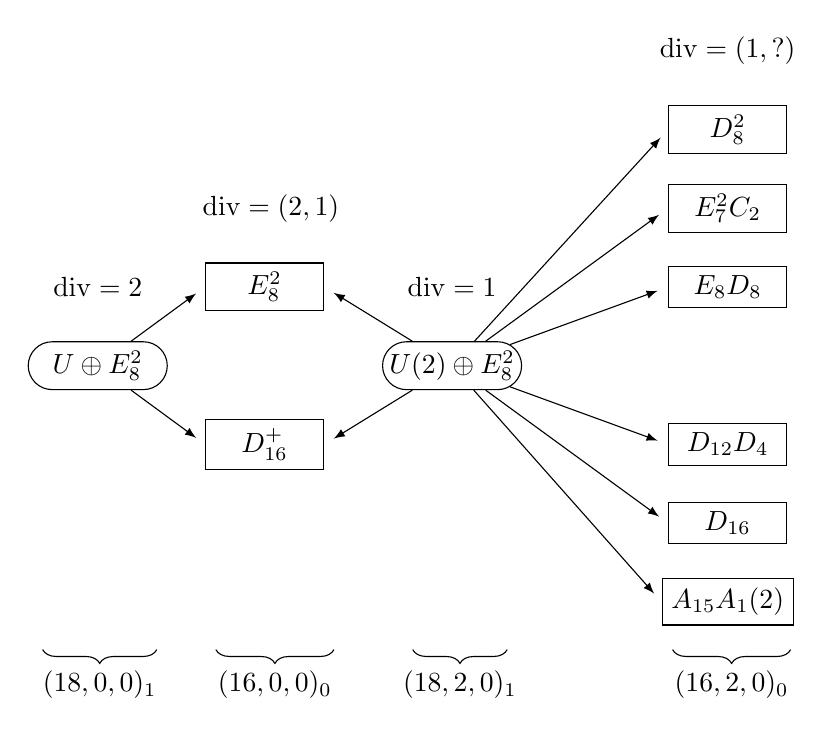
\begin{tikzpicture}

\node[rounded rectangle, draw,minimum width=2cm] (v0) at (0, 0) {$U \oplus E_8^2$};

\node[rectangle, draw,minimum width=1.5cm] (Ca) at (2.12, 1) {$E_8^2$};

\node[rectangle, draw,minimum width=1.5cm] (Cb) at (2.12, -1) {$D_{16}^+$};

\node[rounded rectangle, draw,minimum width=2cm] (v1) at (4.5, 0) {$U(2) \oplus E_8^2$};


\node[rectangle, draw,minimum width=1.5cm] (C1) at (8, 3) {$D_8^2$};
\node[rectangle, draw,minimum width=1.5cm] (C2) at (8, 2) {$E_7^2C_2$};
\node[rectangle, draw,minimum width=1.5cm] (C3) at (8, 1) {$E_8D_8$};

\node[rectangle, draw,minimum width=1.5cm] (C4) at (8, -1) {$D_{12}D_4$};
\node[rectangle, draw,minimum width=1.5cm] (C5) at (8, -2) {$D_{16}$};
\node[rectangle, draw,minimum width=1.5cm] (C6) at (8, -3) {$A_{15}A_1(2)$};

\draw[-latex, shorten >= 0.4em] (v0) to (Ca.west);
\draw[-latex, shorten >= 0.4em] (v0) to (Cb.west);

\draw[-latex, shorten >= 0.4em] (v1) to (Ca.east);
\draw[-latex, shorten >= 0.4em] (v1) to (Cb.east);

\draw[-latex, shorten >= 0.4em] (v1) to (C1.west);
\draw[-latex, shorten >= 0.4em] (v1) to (C2.west);
\draw[-latex, shorten >= 0.4em] (v1) to (C3.west);

\draw[-latex, shorten >= 0.4em] (v1) to (C4.west);
\draw[-latex, shorten >= 0.4em] (v1) to (C5.west);
\draw[-latex, shorten >= 0.4em] (v1) to (C6.west);

\draw [decorate,decoration={brace,amplitude=5pt,mirror,raise=4ex}]
  (-0.7,-3) -- (0.75,-3) node[midway,yshift=-3em]{$(18,0,0)_1$};

\draw [decorate,decoration={brace,amplitude=5pt,mirror,raise=4ex}]
  (1.5,-3) -- (3,-3) node[midway,yshift=-3em]{$(16,0,0)_0$};

\draw [decorate,decoration={brace,amplitude=5pt,mirror,raise=4ex}]
  (4,-3) -- (5.2,-3) node[midway,yshift=-3em]{$(18,2,0)_1$};

\draw [decorate,decoration={brace,amplitude=5pt,mirror,raise=4ex}]
  (7.3,-3) -- (8.8,-3) node[midway,yshift=-3em]{$(16,2,0)_0$};

\node at (0, 1) {$\mathrm{div} = 2$};

\node at (4.5, 1) {$\mathrm{div} = 1$};

\node at (2.2, 2) {$\mathrm{div} = (2, 1)$};

\node at (8, 4) {$\mathrm{div} = (1, ?)$};

\end{tikzpicture}
\caption{}
\label{fig:220-cusp-diagram}
\end{figure}

\end{remark}

\subsection{Coble to Enriques Cusp Correspondence}\label{coble-to-enriques-cusp-correspondence}

\begin{theorem}

The embedding \(\eta: F_{\Co}\to F_{\operatorname{En}}\) induces the correspondence on boundary cusps of the Baily-Borel compactifications shown in \cref{fig:enriques-coble-correspondence}.

\begin{figure}[H]
\centering
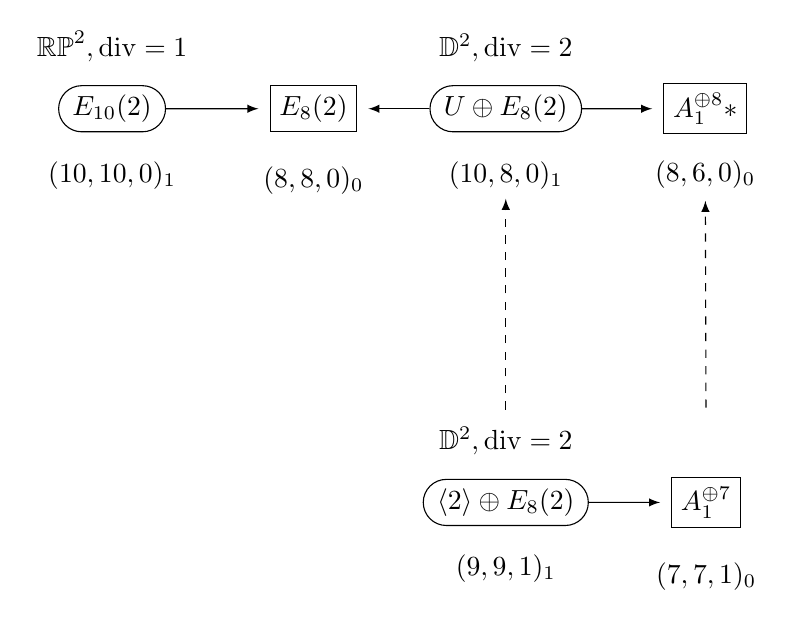
\begin{tikzpicture}
\node [rounded rectangle, draw, label={[label distance=0.75em]-90: $(10,10,0)_1$}, label={[label distance=0.5em]90: $\mathbb{RP}^2, \mathrm{div} = 1$}] (w0) at (0, 0) {$E_{10}(2)$};
\node [rectangle, draw, anchor=west, label={[label distance=0.95em]-90: $(8,8,0)_0$}] (C12) at (2,0) {$E_8(2)$};
\node [rounded rectangle, draw, label={[label distance=0.75em]-90: $(10, 8, 0)_1$}, label={[label distance=0.5em]90: $\mathbb{D}^2, \mathrm{div} = 2$}] (w1) at (5, 0) {$U \oplus E_8(2)$};
\node [rectangle, draw, anchor=west, label={[label distance=0.65em]-90: $(8, 6,  0)_0$}] (C2) at (7,0) {$A_1^{\oplus 8}*$};
%%%%
\draw[-latex, shorten >= 0.4em] (w0) to (C12.west);
\draw[-latex, shorten >= 0.4em] (w1) to (C12.east);
\draw[-latex, shorten >= 0.4em] (w1) to (C2.west);

\node [rounded rectangle, draw, label={[label distance=0.75em]-90: $(9,9,1)_1$}, label={[label distance=0.5em]90: $\mathbb{D}^2, \mathrm{div} = 2$}] (p1) at (5, -5) {$\langle 2 \rangle \oplus E_8(2)$};

\node [rectangle, draw, anchor=west, label={[label distance=0.95em]-90: $(7,7,1)_0$}] (C1) at (7.1,-5) {$A_1^{\oplus 7}$};
\draw[-latex, shorten >= 0.4em] (p1) to (C1.west);
\draw[-latex, shorten >= 2.4em, shorten <= 2.5em, dashed] (p1.north) to (w1.south) ;
\draw[-latex, shorten >= 2.4em, shorten <= 2.5em, dashed] (C1.north) to (C2.south);
\end{tikzpicture}

\caption{Cusp correspondence $F_{\Co} \to F_{\operatorname{En}}$.}
\label{fig:enriques-coble-correspondence}
\end{figure}

\end{theorem}

\begin{remark}

We prove this correspondence by considering divisibilities at the corresponding 0-cusps and 1-cusps in both moduli spaces. We first note that since \(T_{\Co}\) can be written as \(L(2)\) where \(L = \left\langle{1}\right\rangle \oplus E_8\), every \(v\in T_{\Co}\) satisfies \(\operatorname{div}_{T_{\Co}}(v) = 2\).

\end{remark}

\begin{lemma}

\label{lem:divisibility_Tco_one} Fixing notation, \begin{align*}     v_1 &\coloneqq e' & w_1 &\coloneqq\eta(v_1) = \tilde e' \\     v_2 &\coloneqq 2h + \alpha_1 + \alpha_2 & w_2 &\coloneqq\eta(v_2) = 2\tilde e + 2\tilde f + \tilde\alpha_1 + \tilde\alpha_2 \\     J &\coloneqq\left\langle{v_1, v_2}\right\rangle & \tilde J &\coloneqq\left\langle{w_1, w_2}\right\rangle \end{align*} We then have \(\mathrm{div}_{T_{\operatorname{En}} }(w_1) = 2\).

\end{lemma}

\begin{proof}

This follows from the fact that \(\tilde e\in U(2)\) where \(T_{\operatorname{En}} = U \oplus U(2) \oplus E_8(2)\) Noting that \(\tilde e' \tilde f' = 2\), and \(\tilde e'\) is orthogonal to the remaining generators of in the \(U\) and \(E_8(2)\) summands, we thus have \[
\mathrm{div}_{T_{\operatorname{En}} }(w_1) \coloneqq\mathrm{div}_{T_{\operatorname{En}} }(\eta(e'))  
 = \mathrm{div}_{T_{\operatorname{En}} }(\tilde e') = 2
.\] Explicitly, one can check the pairing of \(\tilde e'\) against an arbitrary vector. Write \(x+y+z\in U \oplus U(2)\oplus E_8(2)\), then \[
\tilde e'\cdot(x+y+z) = \tilde e'\cdot y\in \left\{{0, 2}\right\}
\] since \(y\in U(2)\) and \(\tilde e'\in (U\oplus E_8(2))^{\perp T_{\operatorname{En}}}\). Thus \(\beta_{T_{\operatorname{En}}}(\tilde e', T_{\operatorname{En}}) = \beta_{T_{\operatorname{En}}}(\tilde e', U(2)) = 2\bZ\) since \(\tilde e'\cdot\tilde f' = 2\).

\end{proof}

\begin{lemma}

\label{lem:w1_perp_calculation} The 0-cusp \((9,9,1)_1\) in \(F_{\Co}\) maps to the zero-cusp \((10, 8, 0)_1\) in \(F_{\operatorname{En}}\).

\end{lemma}

\begin{proof}

The cusp correspondence follows from computing the lattice \(w_1^{\perp T_{\operatorname{En}}}/\left\langle{w_1}\right\rangle\) under the primitive embedding \(\eta\), since \(\eta(v_1) = w_1\) and \(v_1\) is the isotropic vector corresponding to \((9,9,1)_1\) in \(F_{\Co}\). This particular case follows from a direct computation: \begin{align*} { (\tilde e')^{\perp T_{\operatorname{En}}} \over \left\langle{\tilde e'}\right\rangle } &= { \left\langle{\tilde e,\tilde f}\right\rangle \oplus \left\langle{\tilde e'}\right\rangle \oplus \left\langle{\tilde \alpha_1, \cdots, \tilde \alpha_8}\right\rangle \over \left\langle{\tilde e'}\right\rangle } \\ &\cong \left\langle{\tilde e, \tilde f}\right\rangle \oplus \left\langle{\tilde \alpha_1, \cdots, \tilde \alpha_8}\right\rangle \\ &\cong U \oplus E_{8}(2)  \cong (10,8,0)_1 .\end{align*}

Alternatively, by \cite[Prop. 5.5]{AE22nonsympinv}, the isomorphism type of \(w_1^{\perp T_{\operatorname{En}}}/w_1\) is determined by \(\mathrm{div}_{T_{\operatorname{En}}}(w_1)\); by \cref{lem:divisibility_Tco_one} \(\mathrm{div}_{T_{\operatorname{En}}}(w_1) = 2\). Since the divisibility of the isotropic vector at the Enriques 0-cusp \((10, 8, 0)_1\) is also 2 and the two Enriques 0-cusps are distinguished by divisibility, the correspondence follows.

\end{proof}

\begin{lemma}

\label{lem:1_cusp_correspondence} Cusp \((7,7,1)_0\) in \(F_{\Co}\) maps to cusp \((8, 6, 0)_0\) in \(F_{\operatorname{En}}\).

\end{lemma}

\begin{proof}

The results follows from verifying that the unique orbit \(J\) of a primitive isotropic plane in \(T_{\Co}\) satisfies \(J^{\perp T_{\Co}}/J \cong (7,7,1)\), and identifying the isomorphism type of its image \(\tilde J^{\perp T_{\operatorname{En}}}/\tilde J\) in \(T_{\operatorname{En}}\). One checks that both \(v_2\) and \(w_2\) are isotropic, and \(v_2 \in v_1^{\perp T_{\Co}}/v_1\), and so \(J\) and \(\tilde J\) define isotropic planes in \(T_{\Co}\) and \(T_{\operatorname{En}}\) respectively. By \cite[Prop. 5.5, Lem. 5.9]{AE22nonsympinv}, it suffices to show \[
\mathrm{div}_{w_1^{\perp T_{\operatorname{En}}} /w_1}(w_2)  \coloneqq\mathrm{div}_{U \oplus E_8(2)}(2\tilde e + 2\tilde f + \tilde \alpha_1 + \tilde \alpha_2)= 2
,\] since the isomorphism type of \(\tilde J^\perp/\tilde J\) is uniquely determined by the isomorphism type of \(w_2^{\perp T_{\operatorname{En}}}/w_2\) in \(w_1^{\perp T_{\operatorname{En}}}/w_1\), which is in turn uniquely determined by the characterization of \(w_2\) as odd, even ordinary, or even characteristic in \(w_1^{\perp T_{\operatorname{En}}}/w_1\), which by \cref{lem:w1_perp_calculation} is isomorphic to \(U \oplus E_8(2)\). One checks directly in coordinates: let \(x+y\in U \oplus E_8(2)\) and consider its pairing with \(w_2\): \begin{align*} (x+y)\cdot w_2  = (x+y)\cdot (2\tilde e + 2\tilde f + \tilde \alpha_1 + \tilde \alpha_2 ) = 2x\cdot (\tilde e + \tilde f) + y\cdot (\tilde \alpha_1 + \tilde \alpha_2) ,\end{align*} where we've used orthogonality relations. We note that the first term is evidently even, while the second term is even because all pairings are either zero or divisible by two in the \(E_8(2)\) summand of \(U \oplus E_8(2)\).

\end{proof}

\section{Degenerations of stable Coble surfaces}\label{degenerations-of-stable-coble-surfaces}

\begin{remark}

We describe the KSBA stable limits of Coble surfaces.

\end{remark}

\begin{remark}

We give an example of an integral affine structure for a degeneration of Coble surfaces.

\end{remark}

\section{Appendix}\label{appendix}

\begin{remark}

Following \cite{AEGS23}, a \textbf{Kulikov model} is a \(K\)-trivial semistable model \({\mathcal{X}}\to (C, 0)\) of a degeneration of K3 surfaces over a pointed curve \(C\). For each such degeneration, one can define the dual complex of the central fiber \(\Gamma({\mathcal{X}}_0)\). For Type II degenerations of K3 surfaces, this yields an integral affine \(S^2\) with singularities of total charge \(24\), and for Type III the dual complex is an interval \(\bD^1\). The additional data of an integral affine polarization \(R_{\IA} \subset \Gamma({\mathcal{X}}_0)\) describes the KSBA stable limit of a degeneration \(({\mathcal{X}}^*, \varepsilon \cR^*)\). For Enriques (and hence Coble) surfaces, we take the corresponding dlt models \(\cZ \coloneqq{\mathcal{X}}/\iota_{\operatorname{En}}\) and half-divisor models \((\cZ, \cR_{\cZ}) \coloneqq({\mathcal{X}}, \cR)/\iota_{\operatorname{En}}\) where \({\mathcal{X}}\to (C, 0)\) and \(({\mathcal{X}}, \cR)\) are Kulikov and divisor models of their K3 covers.

\end{remark}

\begin{remark}

The following is a representation of a Type II degeneration -- it is a chain of surfaces whose dual complex is an interval \(\bD^1\), where the ends \(V_1\) and \(V_n\) are rational and the remaining \(V_i\) are isomorphic to \(E\times {\mathbf{P}}^1\) for a fixed elliptic curve \(E\). The intersections \(V_i \cap V_{i+1}\) are double curves isomorphic to \(E\).

\begin{figure}[H]
\centering
\includesvg[width=\textwidth]{inkscape/type-ii-kulikov-degeneration}
\caption{}
\label{fig:typeiikdg}
\end{figure}

A Type III degeneration can be represented by a triangulation of \(S^2\) with singularities, depicted as follows:

\begin{figure}[H]
\centering
\includesvg[width=\textwidth]{inkscape/triangulated-sphere-fan.svg}
\caption{}
\label{fig:triangulated-sphere-fan}
\end{figure}

\end{remark}

\begin{remark}

The following is a combinatorial representation of a Kulikov model for Sterk 2.

\begin{figure}[H]
\centering
\includesvg[width=\textwidth]{inkscape/ias-sterk2-kulikov-model.svg}
\caption{}
\label{fig:ias-sterk2-kulikov-model}
\end{figure}

\end{remark}

\newpage

\printbibliography %Prints bibliography

\end{document}
